
\chapter*{Análisis formal de conceptos}\addcontentsline{toc}{chapter}{Análisis formal de conceptos}

	
	El Análisis Formal de Conceptos (FCA) es una teoría matemática cuyo objetivo es formalizar las nociones de concepto y jerarquía de conceptos, su extracción y análisis.
	
	Usualmente FCA parte de una tabla con información sobre diferentes objetos, la información contenida en esta tabla se procesa realizando un clustering jerárquico que agrupa los objetos en función de sus atributos. Estos clusters son los conceptos que se extraen de la información contenida en la tabla y pueden estar contenidos unos dentro de otros. 
	
	Por ejemplo si partimos de una tabla que contiene animales, todos los animales que posean los atributos \textit{Vive en el agua} y \textit{Vive en la tierra} estarán contenidos en un mismo concepto que sabemos que es \textit{Animal anfibio}.

	
	Este conocimiento puede representarse de diferentes maneras, algunas de las más utilizadas son:
	
	\begin{itemize}
		\item \textbf{Contexto formal}: Es la información de la que parte FCA. Generalmente representado en forma de tabla.
		
		\item  \textbf{Retículo de Conceptos}: un grafo que representa los conceptos como nodos
		y muestra una relación de orden parcial entre ellos (un concepto puede estar contenido dentro de otro).
		
		\item \textbf{Implicación de atributos}: este método de representación consiste en escribir un conjunto de implicaciones entre los atributos del contexto de forma que lo que se expresa es ``Todo objeto que satisface estos atributos, también satisface estos otros''.
	\end{itemize}

	A continuación se describe formalmente en que consiste el \textbf{Análisis formal de conceptos} y sus componentes.
	

\section*{Contextos y conceptos formales}\addcontentsline{toc}{section}{Contextos y conceptos formales}

	
	La unidad básica o fundamental de representación del conocimiento de la que parte FCA es el \textbf{Contexto formal}
	
	\begin{description}
		\item[Contexto Formal] Un contexto formal ($ M $) es una tripleta formada por un conjunto de objetos ($O$), un conjunto de atributos ($A$) y una relación binaria ($I$) entre objetos y atributos ($I \subseteq O \times A $)
	\end{description}

	Esto normalmente se representa como una tabla donde las filas representan los objetos, las columnas los atributos y una cruz en la fila $a$ de la columna $o$ significa que el objeto $o$ esta relacionado con el atributo $a$. Esto puede expresarse como: siendo $o \in O$ y $a \in A$, se dice que $o$ está relacionado con $a$ si $(o, a)\in I$.
	
	\begin{table}
		\centering
		\begin{tabular}{|c||c|c|c|c|c|c|}
			\hline 
			Paises & NW & UNP & CT & G8 & EU & UN \\ 
			\hline 	
			\hline 
			USA & $\times$ & $\times$ &  & $\times$ &  & $\times$ \\ 
			\hline 
			Alemania &  &  &  & $\times$ & $\times$ & $\times$ \\ 
			\hline 
			Francia & $\times$ & $\times$ &  & $\times$ & $\times$ & $\times$ \\ 
			\hline 
			Reino Un. & $\times$ & $\times$ &  & $\times$ & $\times$ & $\times$ \\ 
			\hline 
			Turquía &  &  &  &  &  & $\times$ \\ 
			\hline 
			Qatar &  &  & $\times$ &  &  & $\times$ \\ 
			\hline 
			Italia &  &  & $\times$ & $\times$ & $\times$ & $\times$ \\ 
			\hline 
		\end{tabular} 
		\caption{Contexto formal de paises}
		\label{tabla_paises}
	\end{table}

	Por ejemplo, en el contexto mostrado en el cuadro \ref{tabla_paises} se describe si determinados países pertenecen a organizaciones internacionales (UNP, CT, G8, EU, UN) y si poseen armas nucleares (NW).
	
	Para extraer los conceptos existentes a partir del contexto formal se define primero la operación básica dentro de la teoría de FCA, el \textbf{operador derivación}.
	
	\begin{description}
		\item[Operador derivación] La derivada de un conjunto de atributos $At \subseteq A$ se define como: 
		
		\[ At' = {o \in O | \forall a \in At : (o, a) \in I} \]
		
		Análogamente, la derivada de un conjunto de objetos $Ob \subseteq O$ se define como:
		
		\[ Ob' = {a \in A | \forall o \in Ob : (o, a) \in I} \]
		
	\end{description}

	De forma coloquial, la derivada de un conjunto de atributos es el conjunto de objetos que poseen todos esos atributos y la derivada de un conjunto de objetos es el conjunto de atributos comunes para todos esos objetos.
	
	%Este operador forman una \textit{conexión de Galois} y verifican ciertas propiedades que no entraremos a analizar aquí.
	
	Finalmente a partir de la definición de derivación, se define un \textbf{concepto formal}.
	
	\begin{description}
		\item[Concepto formal] Un concepto formal de un contexto $M = (O,A,I)$ es un par $(Ob,At)$ que cumple
		
		\[ At' = Ob \quad y \quad Ob' = At		\] 
		
		Dado el concepto $C = (Ob, At)$, se denomina: 
		\begin{description}
			\item[Extensión (Ext) del concepto] Conjunto de objetos $Ob$ que lo componen.
			\item[Intensión (Int) del concepto] Conjunto de atributos $At$ del concepto. 
		\end{description}
	\end{description}

	
	Con esto podemos ver que un concepto esta formado por un conjunto de atributos y un conjunto de objetos, tales que los objetos comparten los atributos del conjunto y este conjunto solo contiene los atributos que comparten los objetos.
	
	Algunos de los conceptos que pueden extraerse del contexto formal del cuadro \ref{tabla_paises} son:
	
	\begin{enumerate}
		\item (\{Alemania, Reino Un, Francia, Italia\}, \{EU, G8, UN\}) 
		\item (\{USA, Francia, Reino Un\}, \{NW, UNP, G8, UN\})
		\item (\{USA, Alemania, Francia, Reino Un, Italia\}, \{G8, UN\})

		\item (\{Turquía, USA, Alemania, Qatar, Francia, Reino Un, Italia\}, \{UN\})
	\end{enumerate}
	
	
\section*{Retículo de conceptos}\addcontentsline{toc}{section}{Retículo de conceptos}	

	Antes de definir en que consiste un retículo de conceptos, necesitamos definir las relaciones entre conceptos. La definición de concepto vista anteriormente nos permite definir un orden parcial entre los mismos:
	
	\begin{description}
		\item[Relación de orden] Sea $C_1 = (O_1, A_1)$ y $ C_2 = (O_2, A_2)$, tales que $O_1, O_2 \subseteq O$, $A_1, A_2 \subseteq A$, dos conceptos pertenecientes a un contexto $M = (O,A,I)$. Definimos la relación de orden $ \preceq $ como:
		
		\[ C_1 \preceq C_2 \Longleftrightarrow O_1 \subseteq O_2 \;\; (\Leftrightarrow A_2 \subseteq A_1 ) \]
	
		Se dice que $C_1$ es \textbf{subconcepto} de $C_2$ (o $C_2$ es \textbf{superconcepto} de $C_1$).
	\end{description} 

	 Explicado de forma menos formal, un concepto es subconcepto de otro cuando su conjunto de objetos es un subconjunto de los de el segundo concepto (o lo que es lo mismo, el conjunto de atributos del segundo es un subconjunto de los del primero.). 
	
	Esto establece una relación jerárquica de orden parcial entre los conceptos formales. El conjunto de todos los conceptos de un contexto junto con esta relación de orden forman un retículo completo que se denomina \textbf{Retículo de conceptos} y denotamos como $R(M)$.


	%Completo: que tiene supremo e infimo
	
	Representando gráficamente el retículo podemos leer fácilmente los objetos, atributos y relaciones y ayuda a comprender la estructura de los datos y el contexto. El retículo se representa como un grafo en el que los nodos representan conceptos formales y mediante el etiquetado de los mismos con los atributos y objetos puede calcularse de forma rápida la extensión o intensión de cualquiera de ellos simplemente siguiendo las lineas hacia arriba (intensión) o hacia abajo (extensión).
	
	\begin{figure}
		\centering
		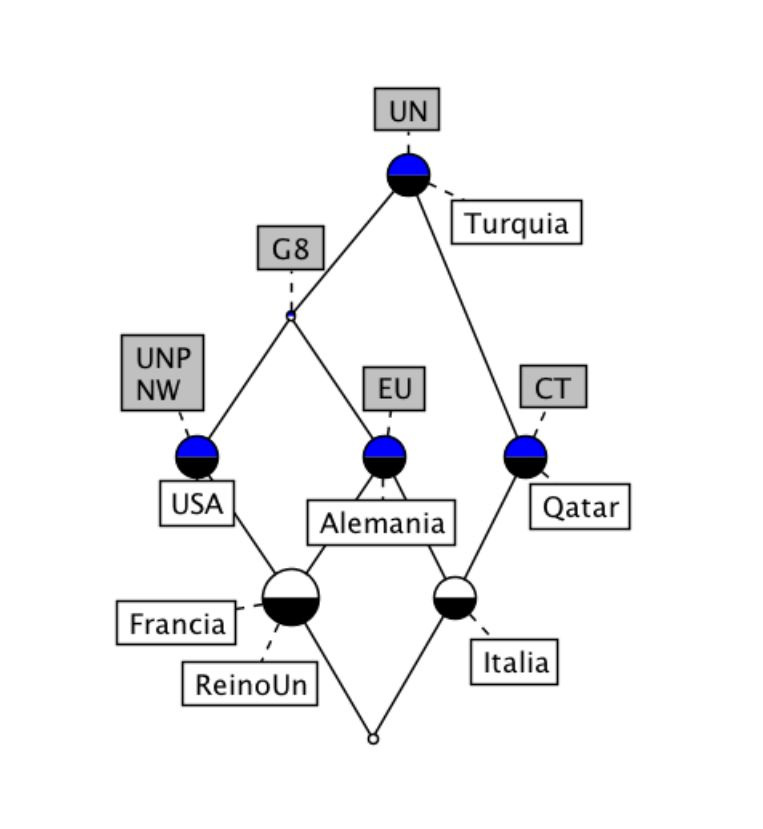
\includegraphics[width=0.5\linewidth]{02_FCA/reticulo}
		\caption{Imagen del retículo}
		\label{reticulo}
	\end{figure}

	En la figura \ref{reticulo} puede verse el retículo correspondiente al contexto formal del cuadro \ref{tabla_paises}.
	
	
	
\section*{Implicación de atributos}\addcontentsline{toc}{section}{Implicación de atributos}

	Otra forma de especificar un contexto formal, y la que nos interesa para nuestro trabajo, es escribiéndolo como un conjunto de implicaciones entre atributos del contexto de forma que el contexto pueda ser reconstruido de forma equivalente partiendo del conjunto de implicaciones. 
	
	Una implicación es una restricción sobre los atributos con la forma: 
	
	\[ \{a_i,...,a_j\} \rightarrow \{a_k,...,a_m\} \]
	
	Lo cual puede leerse como ``Todo objeto que posee los atributos $\{a_i,...,a_j\}$ también posee los atributos $\{a_m,...,a_k\}$''.
	
	La definición formal de una implicación de atributos en FCA es: 
	
	\begin{description}
		\item[Implicación entre atributos] Sea $M = (O,A,I)$ un contexto formal. Una implicación de atributos es un par de conjuntos $L, R \subseteq A$, normalmente escritos $L \rightarrow R$. Una implicación $L \rightarrow R$ es válida en $M$ si para todo objeto de $M$ que tiene todos los atributos de $L$ también tienen todos los atributos de $R$ (todo objeto que no tenga los atributos de $L$ puede tener o no tener los atributos de $R$). Todas las implicaciones extraídas de un contexto $M$ se denotan como $Imp(M)$.
	\end{description}
	
	Algunas implicaciones que pueden extraerse del contexto del cuadro \ref{tabla_paises} son:
	
	\begin{itemize}
		\item $\{\;\} \rightarrow$ UN
		\item CT, G8, UN $\rightarrow$ EU
		\item EU, UN $\rightarrow$ G8 
	\end{itemize}

	 Podemos interpretar estas fórmulas como si pertenecieran a la lógica proposicional y aplicar los algoritmos de razonamiento de la misma. Esto nos permite aplicar la \textbf{retracción conservativa} mencionada en la introducción sobre conjuntos de implicaciones de atributos generados tras la aplicación de FCA a un contexto.
	 
	 Para poder razonar sobre estos conjuntos de reglas se utilizan las reglas de Armstrong para implicaciones: 
	 
	 $
	 	\frac{}{X \to X} (Identidad) \; \frac{X \to Y}{X \cup Z \to Y}(Extension) \; \frac{X \to Y \quad Y \cup Z \to W}{X \cup Z \to W}(Substitucion)
	 $
	
	Mediante la aplicación sucesiva de estas reglas puede realizarse razonamiento hacia delante partiendo de cualquier conjunto de implicaciones.
	
\section*{Retracción aplicada a FCA}\addcontentsline{toc}{section}{Retracción aplicada a FCA} 	

Ya que nuestro objetivo es trabajar con implicaciones de atributos obtenidas en FCA podemos especificar aun más los conceptos descritos en este apartado.

\begin{description}
	\item[Extensión y retracción conservativa] 
	Sea $M = (O,A,I)$ un contexto formal y $\mathcal{L} = Imp(M)$ el conjunto de implicaciones derivado de ese contexto. Se dice que $\mathcal{L}$ es una \textbf{extensión conservativa} de $\mathcal{L}'$ (o que $\mathcal{L}'$ es una \textbf{retracción conservativa} de $\mathcal{L}$) si:
	
	
	Siendo $H = att(\mathcal{L}')$ el conjunto de atributos que aparecen en las implicaciones de $\mathcal{L}'$ y $K = impl(H)$ todas las implicaciones que pueden construirse con el conjunto de atributos $H$, se cumple que: 
	
	
	\[ \mathcal{L} \models \mathcal{L}' \quad y \quad \forall L \in K \;\; [si \ \mathcal{L} \models L \Longrightarrow \mathcal{L}' \models L]  \]

\end{description}

Lo cual significa que dado un conjunto de implicaciones y una retracción conservativa del mismo, cualquier implicación construida utilizando los atributos de la retracción sera cierta en la misma si lo es en el conjunto original.

Una vez que conocemos esta definición queremos ser capaces de construir retracciones conservativas de los conjuntos de implicaciones. Para ello necesitamos definir un operador de olvido. Se pueden definir diferentes operadores de olvido todos ellos válidos desde el punto de vista lógico, pero no todos son válidos para nuestro problema.

Puesto que estamos trabajando sobre la lógica proposicional cualquier operador de olvido válido funcionará con nuestras implicaciones, pero el conjunto resultante de su aplicación no tiene por qué estar limitado a contener únicamente implicaciones. 

Por ello utilizaremos un operador de olvido específicamente creado para esta problemática y cuya validez se demuestra en \cite{retraccion}.


\begin{description}
	\item[Operador de olvido para implicaciones] 
	Sea $C_i = Y_{1}^i \rightarrow Y_{2}^i$  una implicación tal que $Y_{1}^i \cap Y_{2}^i = \emptyset$. El operador $\partial_p (C_1, C_2)$ es un operador de olvido del atributo $p$:
	
	\begin{equation}
	\label{operadorOlvido}
	\partial_p (C_1, C_2) = 			
	\begin{cases} 
	\{C_1, C_2\} & p \notin att(C_1) \cup att(C_2) \\
	\{C_2\} &  p \in Y_1^1, p \notin att(C_2) \\
	\{Y_1^1 \rightarrow (Y_2^1 \, \backslash p) , C_2\} & p \in Y_2^1, p \notin att(C_2) \\
	\{ \top \} & p \in (Y_1^1 \cap Y_1^2) \cup (Y_2^1 \cap Y_2^2) \\
	\{Resolvente_p(C_1, C_2)\} & p \in Y_1^2 \cap Y_2^1
	\end{cases}
	\end{equation}
	
	donde 
	
	\[
	Resolvente_p(C_1, C_2) := \{Y_1^1 \rightarrow Y_2^1 \backslash \{p\}, Y_1^1 \cup (Y_1^2 \backslash \{p\}) \rightarrow Y_2^2 \}
	\]
	
\end{description}

Aplicando este operador sobre todas las combinaciones de implicaciones de un conjunto podemos eliminar un atributo del mismo. Sin embargo este operador es simétrico, es decir $\partial_p (C_1, C_2) = \partial_p (C_2, C_1)$, lo cual nos permite realizar una importante optimización, podemos ignorar todas las combinaciones simétricas pasando de $O(n^2)$ a un $O(n\log(n))$.




	

